\documentclass[12pt,halfline,a4paper,]{ouparticle}

% Packages I think are necessary for basic Rmarkdown functionality
\usepackage{hyperref}
\usepackage{graphicx}
\usepackage{listings}
\usepackage{color}
\usepackage{fancyvrb}
\usepackage{framed}

% For knitr::kable functionality
\usepackage{booktabs}
\usepackage{longtable}

%% To allow better options for figure placement
%\usepackage{float}

% Packages that are supposedly required by OUP sty file
\usepackage{amssymb, amsmath, geometry, amsfonts, verbatim, endnotes, setspace}

% For code highlighting I think
\DefineVerbatimEnvironment{Highlighting}{Verbatim}{commandchars=\\\{\}}
\definecolor{shadecolor}{RGB}{248,248,248}
\newenvironment{Shaded}{\begin{snugshade}}{\end{snugshade}}
\newcommand{\AlertTok}[1]{\textcolor[rgb]{0.94,0.16,0.16}{#1}}
\newcommand{\AnnotationTok}[1]{\textcolor[rgb]{0.56,0.35,0.01}{\textbf{\textit{#1}}}}
\newcommand{\AttributeTok}[1]{\textcolor[rgb]{0.77,0.63,0.00}{#1}}
\newcommand{\BaseNTok}[1]{\textcolor[rgb]{0.00,0.00,0.81}{#1}}
\newcommand{\BuiltInTok}[1]{#1}
\newcommand{\CharTok}[1]{\textcolor[rgb]{0.31,0.60,0.02}{#1}}
\newcommand{\CommentTok}[1]{\textcolor[rgb]{0.56,0.35,0.01}{\textit{#1}}}
\newcommand{\CommentVarTok}[1]{\textcolor[rgb]{0.56,0.35,0.01}{\textbf{\textit{#1}}}}
\newcommand{\ConstantTok}[1]{\textcolor[rgb]{0.00,0.00,0.00}{#1}}
\newcommand{\ControlFlowTok}[1]{\textcolor[rgb]{0.13,0.29,0.53}{\textbf{#1}}}
\newcommand{\DataTypeTok}[1]{\textcolor[rgb]{0.13,0.29,0.53}{#1}}
\newcommand{\DecValTok}[1]{\textcolor[rgb]{0.00,0.00,0.81}{#1}}
\newcommand{\DocumentationTok}[1]{\textcolor[rgb]{0.56,0.35,0.01}{\textbf{\textit{#1}}}}
\newcommand{\ErrorTok}[1]{\textcolor[rgb]{0.64,0.00,0.00}{\textbf{#1}}}
\newcommand{\ExtensionTok}[1]{#1}
\newcommand{\FloatTok}[1]{\textcolor[rgb]{0.00,0.00,0.81}{#1}}
\newcommand{\FunctionTok}[1]{\textcolor[rgb]{0.00,0.00,0.00}{#1}}
\newcommand{\ImportTok}[1]{#1}
\newcommand{\InformationTok}[1]{\textcolor[rgb]{0.56,0.35,0.01}{\textbf{\textit{#1}}}}
\newcommand{\KeywordTok}[1]{\textcolor[rgb]{0.13,0.29,0.53}{\textbf{#1}}}
\newcommand{\NormalTok}[1]{#1}
\newcommand{\OperatorTok}[1]{\textcolor[rgb]{0.81,0.36,0.00}{\textbf{#1}}}
\newcommand{\OtherTok}[1]{\textcolor[rgb]{0.56,0.35,0.01}{#1}}
\newcommand{\PreprocessorTok}[1]{\textcolor[rgb]{0.56,0.35,0.01}{\textit{#1}}}
\newcommand{\RegionMarkerTok}[1]{#1}
\newcommand{\SpecialCharTok}[1]{\textcolor[rgb]{0.00,0.00,0.00}{#1}}
\newcommand{\SpecialStringTok}[1]{\textcolor[rgb]{0.31,0.60,0.02}{#1}}
\newcommand{\StringTok}[1]{\textcolor[rgb]{0.31,0.60,0.02}{#1}}
\newcommand{\VariableTok}[1]{\textcolor[rgb]{0.00,0.00,0.00}{#1}}
\newcommand{\VerbatimStringTok}[1]{\textcolor[rgb]{0.31,0.60,0.02}{#1}}
\newcommand{\WarningTok}[1]{\textcolor[rgb]{0.56,0.35,0.01}{\textbf{\textit{#1}}}}

% For making Rmarkdown lists
\providecommand{\tightlist}{%
  \setlength{\itemsep}{0pt}\setlength{\parskip}{0pt}}

% Part for setting citation format package: natbib

% Part for setting citation format package: biblatex

% Part for indenting CSL refs
% Pandoc citation processing
\newlength{\csllabelwidth}
\setlength{\csllabelwidth}{3em}
\newlength{\cslhangindent}
\setlength{\cslhangindent}{1.5em}
% for Pandoc 2.8 to 2.10.1
\newenvironment{cslreferences}%
  {}%
  {\par}
% For Pandoc 2.11+
\newenvironment{CSLReferences}[3] % #1 hanging-ident, #2 entry spacing
 {% don't indent paragraphs
  \setlength{\parindent}{0pt}
  % turn on hanging indent if param 1 is 1
  \ifodd #1 \everypar{\setlength{\hangindent}{\cslhangindent}}\ignorespaces\fi
  % set entry spacing
  \ifnum #2 > 0
  \setlength{\parskip}{#2\baselineskip}
  \fi
 }%
 {}
\usepackage{calc} % for calculating minipage widths
\newcommand{\CSLBlock}[1]{#1\hfill\break}
\newcommand{\CSLLeftMargin}[1]{\parbox[t]{\csllabelwidth}{#1}}
\newcommand{\CSLRightInline}[1]{\parbox[t]{\linewidth - \csllabelwidth}{#1}}
\newcommand{\CSLIndent}[1]{\hspace{\cslhangindent}#1}
% Pandoc header

\begin{document}

\title{\textbf{Homework assignment title.}}

\author{%
\name{Paco de Lucía}\address{778899}
\and
\name{Baby Yoda}\address{774455}
\and
\name{Chick Corea}\address{884422}
\and
\name{An alternative for big teams - Chick Corea (884422), Baby Yoda
(774455), Paco de Lucía (778899), Suzanne Ciani (365411), Alan Turing
(312511) and others.}
}

\abstract{Summary of main findings and conclusions. Optional section.}

\date{Last compiled on: 07/07/2021, 23:09:08.}

\keywords{quantitative finance; financial risk; financial modeling in
R; Optional section.}

\maketitle



\hypersetup{linkcolor=blue}

\hypertarget{introduction.}{%
\section{Introduction.}\label{introduction.}}

\emph{Look how you can add web links in the following sentence}. This
template is based on the generic OUP template available
\href{https://academic.oup.com/icesjms/pages/General_Instructions}{here}.
\textbf{Now, look how you can add a different font}. This is useful for
\texttt{file} or \texttt{function names}. The original OUP sample tex
document, providing more details on preferred formatting for LaTeX
documents, is included with the template in the file
\texttt{ouparticle\_sample.tex}.

Here are some sample references. \emph{Reference in brackets as in a
list.} Please see (\protect\hyperlink{ref-Hull}{Hull 2015a};
\protect\hyperlink{ref-carhart1997persistence}{Carhart 1997}) for a full
discussion of multi-factor models. Bibliography will appear at the end
of the document. \emph{Second, without brackets, separated by a comma.}
See \protect\hyperlink{ref-Hull}{Hull}
(\protect\hyperlink{ref-Hull}{2015a}),
\protect\hyperlink{ref-Hull2}{Hull}
(\protect\hyperlink{ref-Hull2}{2015b}),
\protect\hyperlink{ref-cochrane2009asset}{Cochrane}
(\protect\hyperlink{ref-cochrane2009asset}{2009}) for a formal
demonstration of analytical results, and
(\protect\hyperlink{ref-carhart1997persistence}{Carhart 1997};
\protect\hyperlink{ref-cochrane1996cross}{Cochrane 1996}) for some
empirical results.

\hypertarget{methodology.}{%
\section{Methodology.}\label{methodology.}}

An equation with a label for cross-referencing:

\begin{equation}\label{eq:eq1}
\int^{r_2}_0 F(r,\varphi){\rm d}r\,{\rm d}\varphi = [\sigma r_2/(2\mu_0)]
\int^{\infty}_0\exp(-\lambda|z_j-z_i|)\lambda^{-1}J_1 (\lambda r_2)J_0
(\lambda r_i\,\lambda {\rm d}\lambda)
\end{equation}

This equation can be referenced as follows: Eq. \ref{eq:eq1}. Now a
simpler equation:

\begin{equation}\label{eq:eq2}
w=\sum^{20}_{i=1}[1/n^i]
\end{equation}

This equation can be referenced as Eq. \ref{eq:eq2}.

We can also write equations within the main text as here:
\(w=\sum^{20}_{i=1}[1/n^i]\).

\hypertarget{a-subsection.}{%
\subsection{A subsection.}\label{a-subsection.}}

A numbered list:

\begin{enumerate}
\def\labelenumi{\arabic{enumi})}
\item
  First numbered point
\item
  Second numbered point

  \begin{itemize}
  \tightlist
  \item
    Subpoint
  \end{itemize}
\end{enumerate}

A bullet list:

\begin{itemize}
\tightlist
\item
  First point
\item
  Second point
\end{itemize}

\hypertarget{results.}{%
\section{Results.}\label{results.}}

\hypertarget{generate-a-figure.}{%
\subsection{Generate a figure.}\label{generate-a-figure.}}

\begin{Shaded}
\begin{Highlighting}[]
\FunctionTok{plot}\NormalTok{(}\DecValTok{1}\SpecialCharTok{:}\DecValTok{10}\NormalTok{, }\AttributeTok{main =} \StringTok{"Some data"}\NormalTok{, }\AttributeTok{xlab =} \StringTok{"Distance (cm)"}\NormalTok{, }
     \AttributeTok{ylab =} \StringTok{"Time (hours)"}\NormalTok{)}
\end{Highlighting}
\end{Shaded}

\begin{figure}[H]
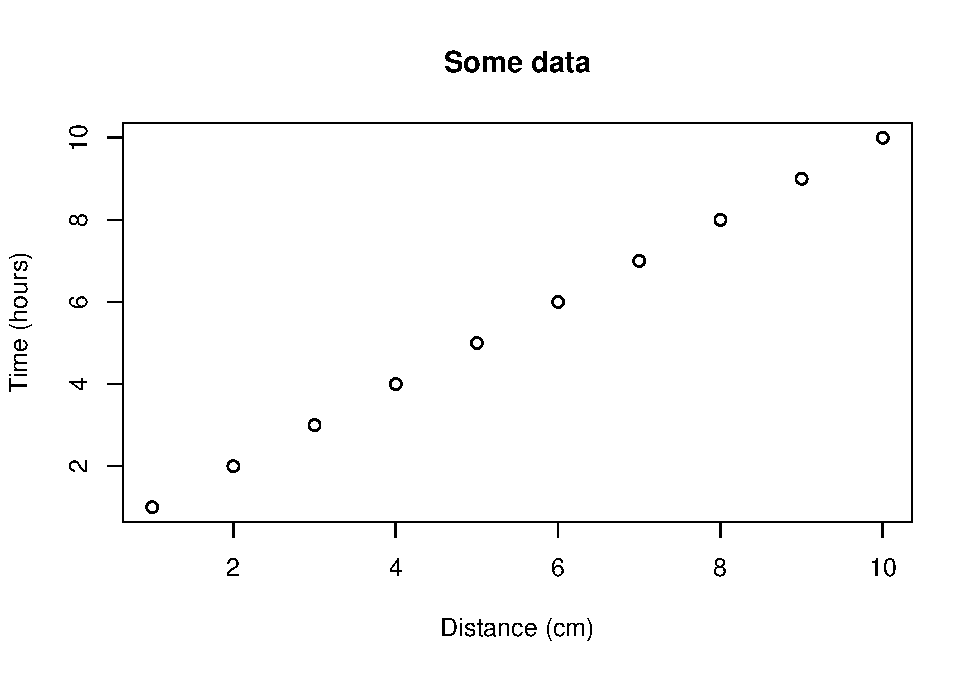
\includegraphics[width=1\linewidth]{assignment_template_files/figure-latex/fig1-1} \caption{This is the first figure.}\label{fig:fig1}
\end{figure}

You can reference this figure as follows: Fig. \ref{fig:fig1}.

\begin{Shaded}
\begin{Highlighting}[]
\FunctionTok{plot}\NormalTok{(}\DecValTok{1}\SpecialCharTok{:}\DecValTok{5}\NormalTok{, }\AttributeTok{pch =} \DecValTok{19}\NormalTok{, }\AttributeTok{main =} \StringTok{"Some data"}\NormalTok{, }\AttributeTok{xlab =} \StringTok{"Distance (cm)"}\NormalTok{, }
     \AttributeTok{ylab =} \StringTok{"Time (hours)"}\NormalTok{)}
\end{Highlighting}
\end{Shaded}

\begin{figure}[H]
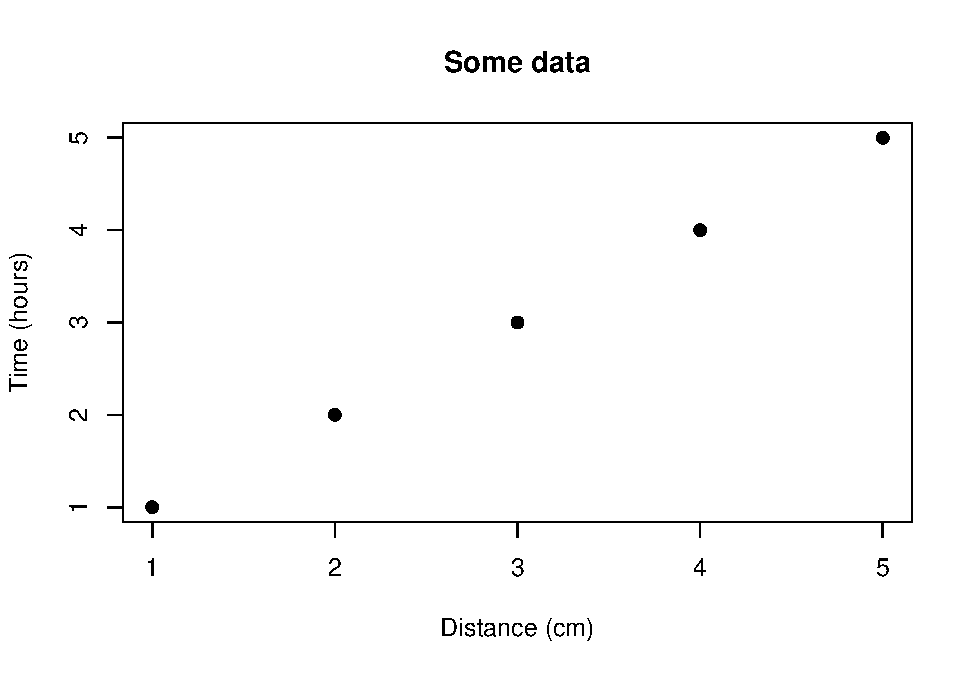
\includegraphics[width=1\linewidth]{assignment_template_files/figure-latex/fig2-1} \caption{This is the second figure.}\label{fig:fig2}
\end{figure}

Reference to second figure: Fig. \ref{fig:fig2}

\hypertarget{generate-a-table-using-xtable.}{%
\subsection{\texorpdfstring{Generate a table using
\texttt{xtable}.}{Generate a table using xtable.}}\label{generate-a-table-using-xtable.}}

\begin{Shaded}
\begin{Highlighting}[]
\NormalTok{df }\OtherTok{=} \FunctionTok{data.frame}\NormalTok{(}\AttributeTok{ID =} \DecValTok{1}\SpecialCharTok{:}\DecValTok{3}\NormalTok{, }\AttributeTok{code =}\NormalTok{ letters[}\DecValTok{1}\SpecialCharTok{:}\DecValTok{3}\NormalTok{])}

\CommentTok{\# Creates tables that follow OUP guidelines using xtable}
\FunctionTok{library}\NormalTok{(xtable) }
\FunctionTok{print}\NormalTok{(}\FunctionTok{xtable}\NormalTok{(df, }\AttributeTok{caption =} \StringTok{"This is the table caption"}\NormalTok{, }
             \AttributeTok{label =} \StringTok{"tab:tab1"}\NormalTok{), }\AttributeTok{comment =} \ConstantTok{FALSE}\NormalTok{)}
\end{Highlighting}
\end{Shaded}

\begin{table}[ht]
\centering
\begin{tabular}{rrl}
  \hline
 & ID & code \\ 
  \hline
1 &   1 & a \\ 
  2 &   2 & b \\ 
  3 &   3 & c \\ 
   \hline
\end{tabular}
\caption{This is the table caption} 
\label{tab:tab1}
\end{table}

You can reference this table as follows: Table \ref{tab:tab1}.

\hypertarget{generate-a-table-using-kable.}{%
\subsection{\texorpdfstring{Generate a table using
\texttt{kable}.}{Generate a table using kable.}}\label{generate-a-table-using-kable.}}

\begin{Shaded}
\begin{Highlighting}[]
\NormalTok{df }\OtherTok{=} \FunctionTok{data.frame}\NormalTok{(}\AttributeTok{ID =} \DecValTok{1}\SpecialCharTok{:}\DecValTok{3}\NormalTok{, }\AttributeTok{code =}\NormalTok{ letters[}\DecValTok{1}\SpecialCharTok{:}\DecValTok{3}\NormalTok{])}

\CommentTok{\# kable can alse be used for creating tables}
\NormalTok{knitr}\SpecialCharTok{::}\FunctionTok{kable}\NormalTok{(df, }\AttributeTok{caption =} \StringTok{"This is the table caption"}\NormalTok{, }\AttributeTok{format =} \StringTok{"latex"}\NormalTok{,}
             \AttributeTok{booktabs =} \ConstantTok{TRUE}\NormalTok{, }\AttributeTok{label =} \StringTok{"tab2"}\NormalTok{)}
\end{Highlighting}
\end{Shaded}

\begin{table}

\caption{\label{tab:tab2}This is the table caption}
\centering
\begin{tabular}[t]{rl}
\toprule
ID & code\\
\midrule
1 & a\\
2 & b\\
3 & c\\
\bottomrule
\end{tabular}
\end{table}

You can reference this table as follows: Table \ref{tab:tab2}.

\hypertarget{conclusion.}{%
\section{Conclusion.}\label{conclusion.}}

You can cross-reference sections and subsections as follows: Section
\ref{methodology.} and Section \ref{a-subsection.}.

\textbf{\emph{Note:}} the last section in the document will be used as
the section title for the bibliography.

\hypertarget{references.}{%
\section*{References.}\label{references.}}
\addcontentsline{toc}{section}{References.}

\hypertarget{refs}{}
\begin{CSLReferences}{1}{0}
\leavevmode\hypertarget{ref-carhart1997persistence}{}%
Carhart, Mark M. 1997. {``On Persistence in Mutual Fund Performance.''}
\emph{The Journal of Finance} 52 (1): 57--82.

\leavevmode\hypertarget{ref-cochrane1996cross}{}%
Cochrane, John H. 1996. {``A Cross-Sectional Test of an Investment-Based
Asset Pricing Model.''} \emph{Journal of Political Economy} 104 (3):
572--621.

\leavevmode\hypertarget{ref-cochrane2009asset}{}%
---------. 2009. \emph{Asset Pricing: Revised Edition}. Princeton
university press.

\leavevmode\hypertarget{ref-Hull}{}%
Hull, John C. 2015a. \emph{Options, Futures, and Other Derivatives}. 9th
ed. Prentice Hall.

\leavevmode\hypertarget{ref-Hull2}{}%
---------. 2015b. \emph{Options, Futures, and Other Derivatives}. 9th
ed. Prentice Hall.

\end{CSLReferences}






\end{document}
